\documentclass[simplex.tex]{subfiles}
% DO NOT INCLUDE PREAMBLES/PACKAGES HERE!!
% packages are inherited from preamble.tex; you can compile this on its own
\begin{document}
\subsection[Randomer Forest]{Randomer Forest (RerF)}

Previously, we had demonstrated that RerF tends to outperform other tree ensemble algorithms on synthetic datasets as well as a large suite of benchmark datasets. Our current effort is to understand when we can expect RerF to win and when we can expect it to lose. As a first step, we have made scatter plots of classification error against two metrics known to be influential in the performance of ensembles: 1) strength of individual weak learners and 2) diversity of weak learners. Below, the plots suggest that strength seems to have a stronger correlation with classification performance than does diversity. RR-RF tends to have lower average tree strength than both RF and RerF. RerF tends to have higher average tree strength than RF.

\begin{figure}[h!]
\begin{cframed}
\centering
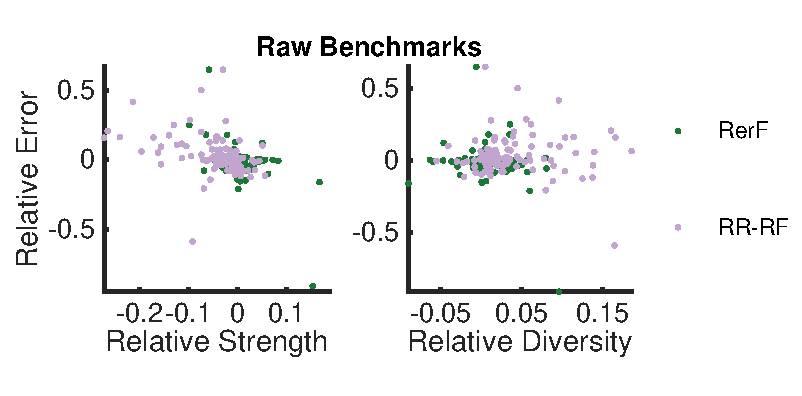
\includegraphics[height=0.30\textheight]{../../figs/PAMI_fig10_strength_diversity_benchmark.pdf}
\caption{
For each of the 114 benchmark datasets, the errors of RerF and RR-RF relative to RF were plotted against 1) the average strength of these algorithms relative to RF (left) and 2) the diversity of trees of these algorithms relative to RF. Tree strength is defined as the individual classification accuracy of a tree. Diversity is defined as the variance in predictions made by the individual trees.
}
\label{fig:RefF3}
\end{cframed}
\end{figure}

The R version of RerF is now functional and is an order of magnitude faster than the Matlab implementation.  This version of RerF allows the user to specify the minimum size of a node and a parameter to tweak the rotation matrix.  Additional basic functionality is being added to this tool including bagging, out-of-bag error reporting, max tree depth, and pruning.  \\



%\clearpage
The R version of Rerf, \href{https://github.com/neurodata/R-RerF}{R-Rerf}, has been tested on a 400Mb artificial dataset.  The training time on this data set is about 3.5 minutes/tree using 1 core, with the training time scaling linearly with the number of cores added.  The increased memory requirements of the multicore implementation are higher than anticipated though -- requiring 8 times the size of the input data per core.  To reduce the memory requirements we are testing depth first vs breadth first tree growing methods.  

\clearpage
\end{document}
